\section{ИССЛЕДОВАНИЕ РАБОТЫ ДЕШИФРАТОРА}

\begin{figure}[H]
	\centering
	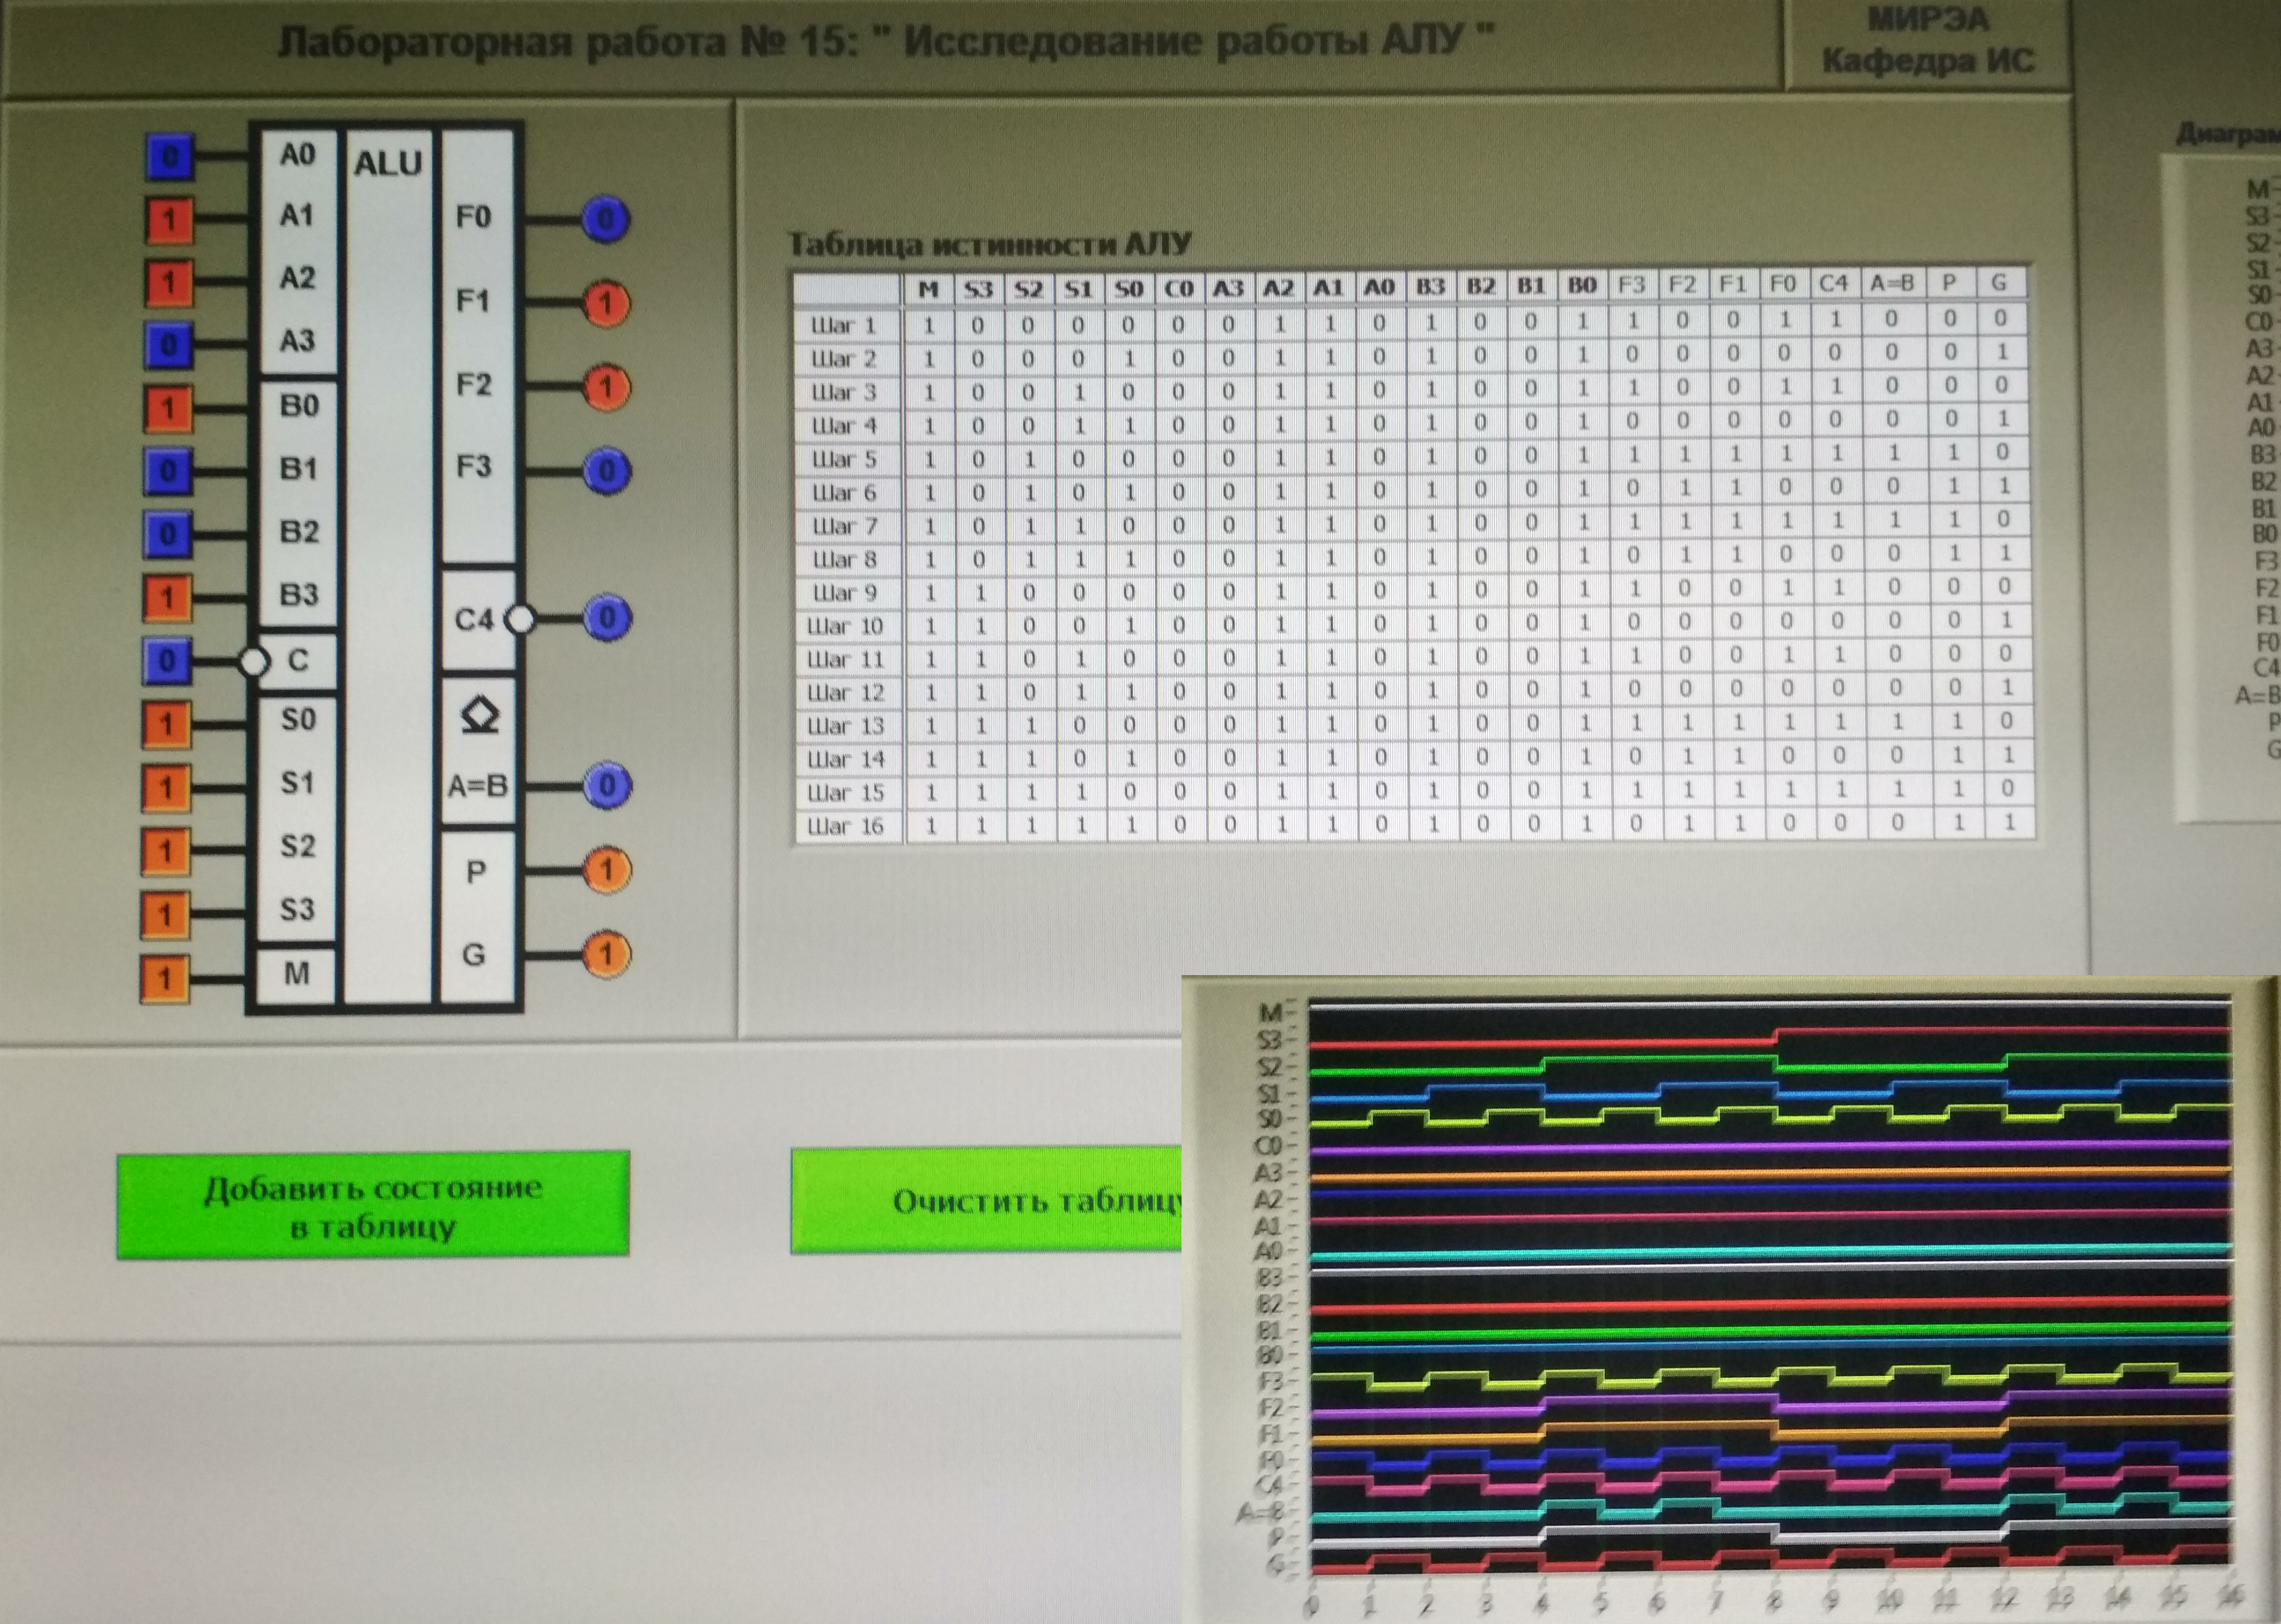
\includegraphics[width=0.95\linewidth]{imgs/3/1}
	\caption{Результат работы дешифратора}
	\label{fig:3_}
\end{figure}

В ходе работы было выяснено, что для работы дешифратора необходимо подать низкий уровень на вход E.
% Шифратор является приоритетным, вход X6 имеет больший приоритет, чем X3

Элемент SN74LV138AT - Low voltage TTL family

Характеристики:

\begin{figure}[H]
	\centering
	\includegraphics[width=0.95\linewidth]{imgs/3/ti1}
	\caption{Схема}
	\label{fig:3_ti1}
\end{figure}

\begin{figure}[H]
	\centering
	\includegraphics[width=0.95\linewidth]{imgs/3/ti2}
	\caption{Максимальные рабочие параметры}
	\label{fig:3_ti2}
\end{figure}

\begin{figure}[H]
	\centering
	\includegraphics[width=0.95\linewidth]{imgs/3/ti3}
	\caption{Рекомендуемые рабочие параметры}
	\label{fig:3_ti3}
\end{figure}

\begin{figure}[H]
	\centering
	\includegraphics[width=0.95\linewidth]{imgs/3/ti4}
	\caption{Электрические характеристики}
	\label{fig:3_ti4}
\end{figure}